\let\negmedspace\undefined
\let\negthickspace\undefined
\documentclass[journal]{IEEEtran}
\usepackage[a5paper, margin=10mm, onecolumn]{geometry}
%\usepackage{lmodern} % Ensure lmodern is loaded for pdflatex
\usepackage{tfrupee} % Include tfrupee package

\setlength{\headheight}{1cm} % Set the height of the header box
\setlength{\headsep}{0mm}     % Set the distance between the header box and the top of the text

\usepackage{gvv-book}
\usepackage{gvv}
\usepackage{cite}
\usepackage{amsmath,amssymb,amsfonts,amsthm}
\usepackage{algorithmic}
\usepackage{graphicx}
\usepackage{textcomp}
\usepackage{cancel}
\usepackage{xcolor}
\usepackage{txfonts}
\usepackage{listings}
\usepackage{enumitem}
\usepackage{mathtools}
\usepackage{gensymb}
\usepackage{comment}
\usepackage[breaklinks=true]{hyperref}
\usepackage{tkz-euclide} 
\usepackage{listings}
% \usepackage{gvv}                                        
\def\inputGnumericTable{}                   
\usepackage[latin1]{inputenc}                                
\usepackage{color}                                            
\usepackage{array}                                     
\usepackage{longtable}                                       
\usepackage{calc}                                     
\usepackage{multirow}                                         
\usepackage{hhline}                                            
\usepackage{ifthen}                                           
\usepackage{lscape}
\begin{document}

\bibliographystyle{IEEEtran}
\title{4.13.53}
\author{EE25BTECH11049 - Sai Krishna Bakki}
\maketitle
\vspace{-3em}
\textbf{Question}\\
Lines $L_1 \equiv ax + by + c = 0$ and $L_2 \equiv lx + my + n = 0$ intersect at the point P and make an angle $\theta$ with each other. Find the equation of a line $L$ different from $L_2$ which passes through P and makes the same angle $\theta$ with $L_1$.

\textbf{Solution}\\
The intersection of lines is given as
\begin{align}
L \equiv L_1 + k L_2 = 0
\end{align}

If $L$ is the reflection of $L_2$ in $L_1$, then for any point \textbf{Q} that lies on $L_2$, its reflection \textbf{R} across the line $L_1$ must lie on $L$.

\begin{align}
 L_1 \equiv ax + by + c = 0 \implies \vec{n}_1^T \vec{x} + c = 0, \vec{n}_1 = \myvec{ a \\ b}.\\
L_2 \equiv lx + my + n = 0 \implies \vec{n}_2^T \vec{x} + n = 0, \vec{n}_2 = \myvec{ l \\ m}. \\
L \equiv (ax+by+c) + k(lx+my+n) = 0 \implies (\vec{n}_1^T \vec{x} + c) + k(\vec{n}_2^T \vec{x} + n) = 0.
\end{align}

Let us choose an arbitrary point Q, with position vector $\vec{q}$, that lies on the line $L_2$. The condition that Q is on $L_2$ is:
\begin{align}
\vec{n}_2^T \vec{q} + n = 0
\label{eq:q_on_l2}
\end{align}
Next, we find the position vector $\vec{r}$ for the point R, which is the reflection of Q in the line $L_1$. The standard vector formula for this reflection is:
\begin{align}
\vec{r} = \vec{q} - 2 \brak{ \frac{\vec{n}_1^T \vec{q} + c}{\vec{n}_1^T \vec{n}_1} } \vec{n}_1
\label{eq:reflection_formula}
\end{align}
According to our principle, the reflected point R must lie on the line $L$. We substitute the expression for its position vector $\vec{r}$ from $\eqref{eq:reflection_formula}$ directly into the equation for $L$.
\begin{align}
(\vec{n}_1^T \vec{r} + c) + k(\vec{n}_2^T \vec{r} + n) = 0\\
    % Full substitution
     \sbrak{ \vec{n}_1^T \brak{ \vec{q} - 2 \frac{\vec{n}_1^T \vec{q} + c}{\vec{n}_1^T \vec{n}_1} \vec{n}_1 } + c } + k \sbrak{ \vec{n}_2^T \brak{ \vec{q} - 2 \frac{\vec{n}_1^T \vec{q} + c}{\vec{n}_1^T \vec{n}_1} \vec{n}_1 } + n } = 0 \\
    % Expand terms
    \implies  \sbrak{ \vec{n}_1^T\vec{q} - 2 \frac{\vec{n}_1^T \vec{q} + c}{\cancel{\vec{n}_1^T \vec{n}_1}} (\cancel{\vec{n}_1^T\vec{n}_1}) + c } + k \sbrak{ (\vec{n}_2^T \vec{q} + n) - 2 \frac{\vec{n}_1^T \vec{q} + c}{\vec{n}_1^T \vec{n}_1} (\vec{n}_2^T\vec{n}_1) } = 0 \\
    % Simplify and use condition
    \implies  \sbrak{ \vec{n}_1^T\vec{q} - 2(\vec{n}_1^T \vec{q} + c) + c } + k \sbrak{ 0 - 2 \frac{(\vec{n}_1^T \vec{q} + c)(\vec{n}_1^T\vec{n}_2)}{\vec{n}_1^T \vec{n}_1} } = 0 && \text{(using \eqref{eq:q_on_l2})} \\
    % Final simplified form
    \implies  -(\vec{n}_1^T \vec{q} + c) - k \sbrak{ 2 \frac{(\vec{n}_1^T \vec{q} + c)(\vec{n}_1^T \vec{n}_2)}{\vec{n}_1^T \vec{n}_1} } = 0
\end{align}


Assuming Q is not on $L_1$, the term $(\vec{n}_1^T \vec{q} + c)$ is non-zero, allowing us to divide the entire equation by it:
\begin{align}
-1 - k \sbrak{ \frac{2(\vec{n}_1^T \vec{n}_2)}{\vec{n}_1^T \vec{n}_1} } = 0\\
k = - \frac{\vec{n}_1^T \vec{n}_1}{2(\vec{n}_1^T \vec{n}_2)}
\end{align}

\subsection*{Final Equation}
Substitute this value of $k$ back into the equation $L_1 + k L_2 = 0$
\begin{align}
L_1 - \frac{\vec{n}_1^T \vec{n}_1}{2(\vec{n}_1^T \vec{n}_2)} L_2 = 0\\
2(\vec{n}_1^T \vec{n}_2) L_1 - (\vec{n}_1^T \vec{n}_1) L_2 = 0
\end{align}
Finally, substituting the algebraic forms for the scalar products:
\begin{itemize}
    \item $\vec{n}_1^T \vec{n}_2 = al + bm$
    \item $\vec{n}_1^T \vec{n}_1 = a^2 + b^2$
\end{itemize}
We arrive at the final equation for the line $L$:
\begin{align}
\boxed{2\myvec{a&b}\myvec{l\\m}\brak{\myvec{a&b}\vec{x}+c} - \myvec{a&b}\myvec{a\\b}\brak{\myvec{l&m}\vec{x}+n} = 0}
\end{align}
\newpage
 \begin{figure}
    \centering
    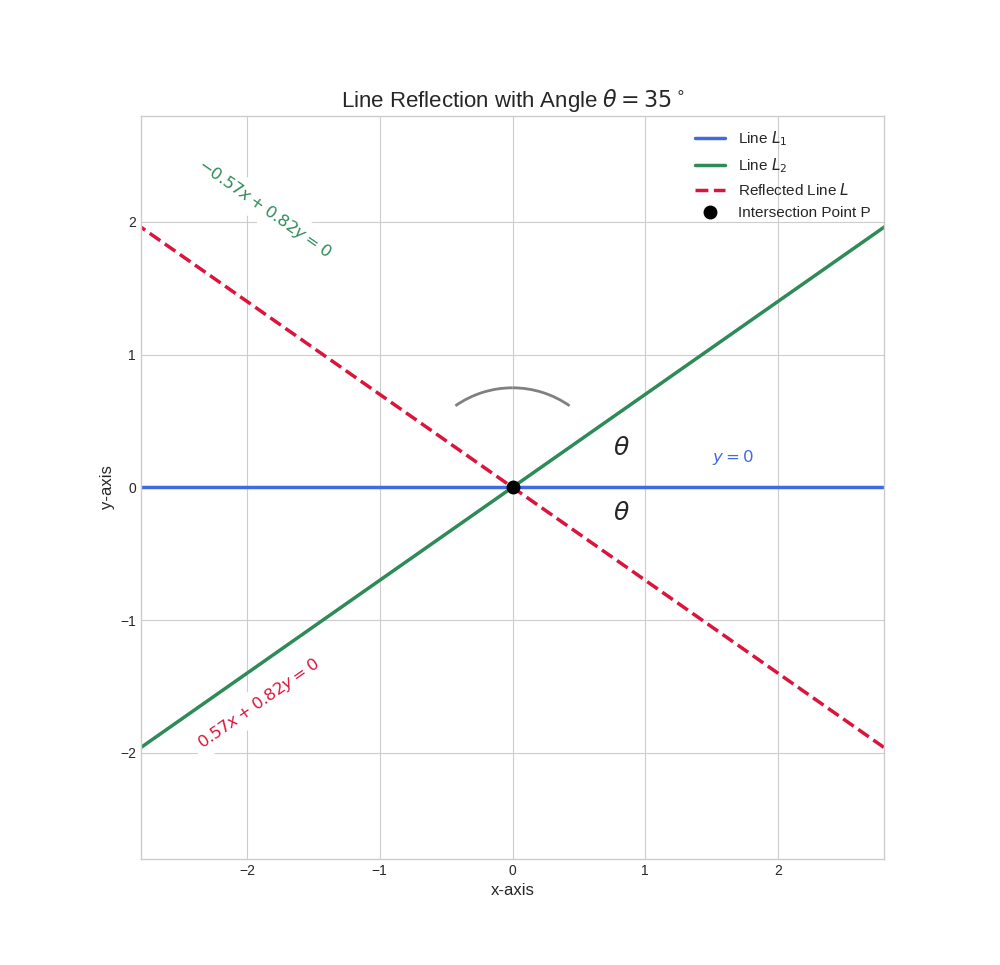
\includegraphics[width=0.9\columnwidth]{figs/Figure_1.png}
    \label{fig:placeholder}
    \caption{}
\end{figure}
\end{document}
